\documentclass[12pt,letterpaper,titlepage]{article}

%% Language and font encodings
\usepackage[english]{babel}
\usepackage[utf8x]{inputenc}
\usepackage[T1]{fontenc}
\usepackage{caption}
%% Sets page size and margins
%%\usepackage[a4paper,top=3cm,bottom=2cm,left=3cm,right=3cm,marginparwidth=1.75cm]{geometry}

%% Useful packages
\usepackage{amsmath}
\usepackage{graphicx}
\usepackage[colorinlistoftodos]{todonotes}
\usepackage[colorlinks=true, allcolors=blue]{hyperref}
\usepackage{physics}

\title{Project 1: Numerical Modeling of 1-D 1-Phase Radial Flow}
\author{Abdullah A. Alghamdi}


\begin{document}
\maketitle

\renewcommand{\abstractname}{Executive Summary}
\begin{abstract}
Numerical simulation is the main method that the industry utilize to predict reservoir performance. This paper will investigate various methods to model 1-D radial flow in a single phase reservoir. The simulation model will consist of 1 well and a cylindrical reservoir. Effects of number of simulation cells on the accuracy of the pressure distribution was discussed. Furthermore, pressure distribution changes over time in both transit and steady state flow were investigated using numerical and analytical methods. Last but not least, rate forecast using 3 different calculation methods, namely numerical and analytical for both transit and steady state flow, were compared. The objective of the paper is to build a numerical simulator and then asses its performance by comparing its outputs to analytically calculated outputs.  
\end{abstract}
\tableofcontents
\pagebreak
\section{Model Preparation}
\subsection{Model Description}
An oil reservoir is approximated by 1-D cylindrical formation of one layer, with a constant thickness of $h=50 \,\text{ft}$, as shown in Figure~\ref{fig:1}. The reservoir has radius of $r_e=1500 \,\text{ft}$ where the well bore radius is $r_w=0.25 \,\text{ft}$. The formation is homogeneous with porosity of $\phi=0.2$, permeability of $k=10 \,\text{mD}$, and compressibility of $c_\phi=1\times10^{-5} \,\text{psi}^{-1}$. Before any oil was flown out of the well, the initial reservoir pressure was $P\mid_{t=0}=3000 \,\text{psi}$.\linebreak
As for fluid properties, the under-saturated oil has a viscosity of $\mu=2 \,\text{cp}$, formation volume factor of $B_o=0.25 \,\text{RB/STB}$, and is slightly compressible  $c_o=2\times10^{-5} \,\text{psi}^{-1}$. Since the reservoir contains single phase fluid, relative permeability and capillary pressure effects are not considered.

\begin{figure}[h]
\centering
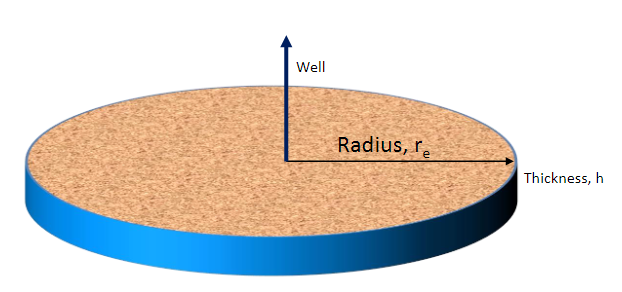
\includegraphics[width=.8\textwidth]{Capture.PNG}
\caption{\label{fig:1}Reservoir model description}
\end{figure}

\subsection{Radial Flow Equation and Boundary Conditions }
radial flow can be modeled using diffusivity equation (see equation \ref{eq:1})
which is derived by using mass conservation and Darcy's law. The derivation of this equation includes significant assumptions that have to be mentioned. It is assumed that:
\begin{itemize}
\item mass conservation is applicable,
\item Darcy law is applicable,
\item fluid is slightly compressible,
\item pressure gradient ($\dv{P}{r}$) is small
\item compressibility $C_o$ and $C_\phi$ are constants,
\item permeability $k$ is independent of pressure and radius,
\item permeability is isotropic,
\item viscosity $\mu$ is independent of pressure and radius,
\item porosity $\phi$ is independent of pressure and radius,
\item thickness $h$ is constant.
\item system contains one phase fluid,
\item now vertical flow ($k_z=0$).
\item gravity and capillary pressure effects are ignored
\end{itemize}

\begin{equation}\label{eq:1}
\frac{1}{r}\pdv{}{r}\left[r\pdv{P}{r}\right] = 158\,\alpha \pdv{P}{t}
\end{equation}
where $$\alpha=\frac{\mu \phi (c_o+c_\phi)}{k}$$
Initial condition:
\begin{equation}
P(r,t)\mid_{t=0}=P_i=3000\,\text{psi}
\end{equation}
Constant Pressure Boundary Conditions:
\begin{align}
P(r,t)\mid_{r=r_e}=&P_e=3000\,\text{psi}\\
P(r,t)\mid_{r=r_w}=&P_{wf}=1000\,\text{psi}
\end{align}
Closed Outer Boundary Conditions:
\begin{equation}
r\dv{P}{r}\mid_{r=r_e}=0\\
\end{equation}
Constant Rate Inner Boundary Conditions:
\begin{equation}
r\dv{P}{r}\mid_{r=r_e}=141.2\frac{qB_o\mu}{kh}\\
\end{equation}
\subsection{Transformation}
The bulk of the pressure changes in radial flow occurs just near the well-bore with pressure changes decreases as the distance from the well-bore increases. Thus to capture these changes, a small $\Delta r$ should be used. However, the smaller the $\Delta r$, the more computing resources are needed. Therefore, several transformation methods can be used to increase the simulation efficiency without losing vital information in the process. In this paper, we will discuss transforming the radial flow equation to the $\chi$ domain where $\chi=\ln{r}$.
\begin{equation*}
\tag{\ref{eq:1}}
\frac{1}{r}\pdv{}{r}\left[r\pdv{P}{r}\right] = 158\, \alpha \pdv{P}{t}
\end{equation*}
Let $$\chi=\ln{(r)}\qquad \Rightarrow \qquad r=e^{\chi}\\$$
\begin{gather*}
\frac{1}{e^{\chi}}\pdv{}{\chi}\left[e^{\chi}\pdv{P}{\chi}\pdv{\chi}{r}\right] \pdv{\chi}{r}= 158\, \alpha \pdv{P}{t} \\
\frac{1}{e^{\chi}}\frac{1}{e^{\chi}}\pdv{}{\chi}\left[\pdv{P}{\chi}\right] =158\,  \alpha \pdv{P}{t}\\
\end{gather*}
\begin{equation}\label{eq:2}
\pdv[2]{P}{\chi} = 158\, e^{2\chi}\alpha \pdv{P}{t} 
\end{equation} 
Transforming initial condition:
\begin{equation}
P(\chi,t)\mid_{t=0}=P_i=3000\,\text{psi}
\end{equation}
Transforming constant pressure boundary conditions:
\begin{gather}
P(\chi,t)\mid_{\chi=\chi_e}=P_e=3000\,\text{psi}\\
P(\chi,t)\mid_{\chi=\chi_w}=P_{wf}=1000\,\text{psi}
\end{gather}
Transforming closed outer boundary conditions:
\begin{equation}
\dv{P}{\chi}\mid_{\chi=\ln{r_e}}=0\\
\end{equation}
Transforming constant rate inner boundary conditions:
\begin{equation}
\dv{P}{\chi}\mid_{\chi=\ln{r_e}}=141.2\frac{qB_o\mu}{kh}\\
\end{equation}
\subsection{Discretization}
Using block-centered implicit discretization to discretize equation \ref{eq:2}:
\begin{gather}
\frac{P^{n+1}_{i-1}-2P^{n+1}_{i}+P^{n+1}_{i+1}}{\Delta\chi^2}= e^{2\chi}\alpha \frac{P^{n+1}_{i}-P^{n}_{i}}{\Delta t}\\
{P^{n+1}_{i-1}-2P^{n+1}_{i}+P^{n+1}_{i+1}} =\frac{\Delta\chi^2e^{2\chi}\alpha}{\Delta t} {P^{n+1}_{i}-P^{n}_{i}}\\
{P^{n+1}_{i-1}-[2+\frac{\Delta\chi^2e^{2\chi}\alpha}{\Delta t}]P^{n+1}_{i}+P^{n+1}_{i+1}} =-\frac{\Delta\chi^2e^{2\chi}\alpha}{\Delta t} P^n_i\label{eq:3}
\end{gather}
to simplify equation \ref{eq:3}:\\
%since $P^n_i=P\mid_{t=0}$
\begin{equation}
a{P^{n+1}_{i-1}+b P^{n+1}_{i}+c P^{n+1}_{i+1}} =d
\end{equation}
where 
\begin{align*}
a &=1\\
b &=-[2+\frac{\Delta\chi^2e^{2\chi}\alpha}{\Delta t}]\\
c &=1\\
d &=-\frac{\Delta\chi^2e^{2\chi}\alpha}{\Delta t}P^n_i\\
\end{align*}
\section{Scenario 1: 4 cells and 1 time step}

In the first scenario, the flow path will be divided to 4 center blocks cells ($N=4$) with spacing of $\Delta\chi$ as shown in Figure \ref{fig:2}. This simulation instance will be limited to 1 time step of 1 day ($t=1$ and $\Delta t=1$). 
\begin{gather}\label{eq:dx}
\Delta\chi=\frac{\ln{r_e}-\ln{r_w}}{n}\\\label{eq:dx2}
\chi_i=\ln{r_w}+\frac{2i-1}{2}\Delta\chi\\\label{eq:dx3}
\chi_N=\ln{r_e}-\frac{1}{2}\Delta\chi
\end{gather}
\begin{table}[h]
\centering
\begin{tabular}{lrrr}
$i$  & $\chi_i$ [ft]& Radius ($r_i$) [ft]  \\\hline
0 &-1.3863 & 0.25\\
1& -0.2989 & 0.74\\
2& 1.8760 & 6.53\\
3 &4.0509 & 57.4\\
4& 6.2258 & 505.6\\
5& 7.3132 & 1500\\
\hline
\end{tabular}
\caption{\label{tab:4}$\chi_i$ and $r_i$ for $i=0-5$}
\end{table}

\begin{figure}[h]
\centering
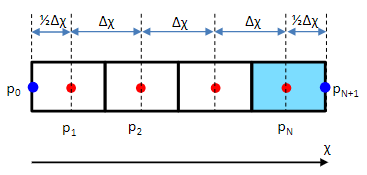
\includegraphics[width=0.7\textwidth]{Capture2.PNG}
\caption{\label{fig:2}Schematic of simulation cells}
\end{figure}
Using Equation \ref{eq:3}, and setting $P^n_i=P\mid_{t=0}$, we find:
\\\underline{when $i=1$:}\\
Since $\Delta\chi$ are not equal on both sides of $P_1$:
\begin{equation}
\frac{\Delta\chi_1P^{n+1}_0-(\Delta\chi_0+\Delta\chi_1)P^{n+1}_1+\Delta\chi_0P^{n+1}_2}{0.5\Delta\chi_0\Delta\chi_1(\Delta\chi_0+\Delta\chi_1)}= e^{2\chi_1}\alpha \frac{P^{n+1}_1-P\mid_{t=0}}{\Delta t}\end{equation}
Since \boxed{$$\Delta\chi_0=\frac{1}{2}\Delta\chi_1$$}
\begin{gather*}
\frac{\Delta\chi_1P^{n+1}_0-\frac{3}{2}\Delta\chi_1P^{n+1}_1+\frac{1}{2}\Delta\chi_1P^{n+1}_2}{\frac{3}{8}\Delta\chi_1^3}= e^{2\chi}\alpha \frac{P^{n+1}_1-P\mid_{t=0}}{\Delta t}\\
8  P^{n+1}_0 -12 P^{n+1}_1 + 4 P^{n+1}_2= \frac{3\Delta\chi^2 e^{2\chi}\alpha}{\Delta t} (P^{n+1}_1-P\mid_{t=0})
\end{gather*}
Since $P_0=P_{wf}$
\begin{equation}\label{eq:i1}
-[12+\frac{3\Delta\chi^2 e^{2\chi_1}\alpha}{\Delta t}]P^{n+1}_1 + 4 P^{n+1}_2= -\frac{3\Delta\chi^2 e^{2\chi_1}\alpha}{\Delta t}P\mid_{t=0}-8  P_{wf} 
\end{equation}

 \underline{when $i=2$:}
\begin{equation}\label{eq:i2}
{P^{n+1}_1-[2+\frac{\Delta\chi^2e^{2\chi}\alpha}{\Delta t}]P^{n+1}_{2}+P^{n+1}_{3}} =-\frac{\Delta\chi^2e^{2\chi_2}\alpha}{\Delta t} P\mid_{t=0}
\end{equation}

 \underline{when $i=3$:}
\begin{equation}\label{eq:i3}
{P^{n+1}_2-[2+\frac{\Delta\chi^2e^{2\chi}\alpha}{\Delta t}]P^{n+1}_{3}+P^{n+1}_{4}} =-\frac{\Delta\chi^2e^{2\chi_3}\alpha}{\Delta t} P\mid_{t=0}
\end{equation}
 \underline{when $i=4$:}\\
Since $\Delta\chi$ are not equal on both sides of $P_4$:
\begin{equation}
\frac{\Delta\chi_4P^{n+1}_3-(\Delta\chi_4+\Delta\chi_34)P^{n+1}_4+\Delta\chi_3P^{n+1}_5}{0.5\Delta\chi_4\Delta\chi_3(\Delta\chi_4+\Delta\chi_3)}= e^{2\chi_4}\alpha \frac{P^{n+1}_4-P\mid_{t=0}}{\Delta t}\end{equation}
Since \boxed{$$\Delta\chi_4=\frac{1}{2}\Delta\chi_3$$}
\begin{gather*}
\frac{\frac{1}{2}\Delta\chi_3P^{n+1}_3-\frac{3}{2}\Delta\chi_3P^{n+1}_4+\Delta\chi_3P^{n+1}_5}{\frac{3}{8}\Delta\chi_3^3}= e^{2\chi_4}\alpha \frac{P^{n+1}_4-P\mid_{t=0}}{\Delta t}\\
4  P^{n+1}_3 -12 P^{n+1}_4 + 8 P^{n+1}_5= \frac{3\Delta\chi^2 e^{2\chi}\alpha}{\Delta t} (P^{n+1}_1-P\mid_{t=0})
\end{gather*}
Since $P_5=P_{e}$ 
\begin{equation}\label{eq:i4}
4 P^{n+1}_3-[12+\frac{3\Delta\chi^2 e^{2\chi_1}\alpha}{\Delta t}]P^{n+1}_4 = -\frac{3\Delta\chi^2 e^{2\chi_1}\alpha}{\Delta t}P\mid_{t=0}-8  P_{e} 
\end{equation}

\renewcommand{\arraystretch}{2}
 \[ \begin{aligned}
    & \begin{bmatrix} 
     -[12+\frac{3\Delta\chi^2 e^{2\chi_1}\alpha}{\Delta t}] & 4 & 0 & 0 \\ 
     1 & -[2+\frac{\Delta\chi^2 e^{2\chi_2}\alpha}{\Delta t}] & 1 & 0 \\
        0 &  1 & -[2+\frac{\Delta\chi^2 e^{2\chi_3}\alpha}{\Delta t}] & 1 \\
       0&0&4& -[12+\frac{3\Delta\chi^2 e^{2\chi_4}\alpha}{\Delta t}]
 \end{bmatrix} 
  \times \begin{bmatrix} 
      P^{n+1}_1        \\ 
      P^{n+1}_2        \\ 
      P^{n+1}_3        \\ 
      P^{n+1}_4        \\ 
    \end{bmatrix} \\&= \left[\begin{array}{l}  -\frac{3\Delta\chi^2 e^{2\chi_1}\alpha}{\Delta t}P\mid_{t=0}-8  P_{wf}\\-\frac{\Delta\chi^2e^{2\chi_2}\alpha}{\Delta t} P\mid_{t=0}\\-\frac{\Delta\chi^2e^{2\chi_3}\alpha}{\Delta t} P\mid_{t=0}\\ -\frac{3\Delta\chi^2 e^{2\chi_4}\alpha}{\Delta t}P\mid_{t=0}-8  P_{e}  \end{array}\right]
\end{aligned}  \] 

The above matrix is a tridiagonal matrix that can be solved using Thomas Algorithm:

\renewcommand{\arraystretch}{2}
 \[ \begin{aligned}
    & \begin{bmatrix} 
     b_1 & c_1 & 0 & 0 \\ 
     a_2 & b_2 & c_2 & 0 \\
        0 &  a_3 & b_3 & c_3 \\
       0&0&a_4& b_4
 \end{bmatrix} 
  \times \begin{bmatrix} 
      P^{n+1}_1        \\ 
      P^{n+1}_2        \\ 
      P^{n+1}_3        \\ 
      P^{n+1}_4        \\ 
    \end{bmatrix} &= \left[\begin{array}{l}  d_1\\d_2\\d_3\\d_4  \end{array}\right]
\end{aligned}  \] 
where
\begin{align*}
a&=\left[0,1,1,4\right]\\
b&=\left[-[12+\frac{3\Delta\chi^2 e^{2\chi_1}\alpha}{\Delta t}], -[2+\frac{\Delta\chi^2 e^{2\chi_2}\alpha}{\Delta t}], -[2+\frac{\Delta\chi^2 e^{2\chi_3}\alpha}{\Delta t}], -[12+\frac{3\Delta\chi^2 e^{2\chi_4}\alpha}{\Delta t}]\right]\\
c&=[4,1,1]\\
d&=\left[-\frac{3\Delta\chi^2 e^{2\chi_1}\alpha}{\Delta t}P\mid_{t=0}-8  P_{wf}, -\frac{\Delta\chi^2e^{2\chi_2}\alpha}{\Delta t} P\mid_{t=0}, -\frac{\Delta\chi^2e^{2\chi_3}\alpha}{\Delta t} P\mid_{t=0}, -\frac{3\Delta\chi^2 e^{2\chi_4}\alpha}{\Delta t}P\mid_{t=0}-8  P_{e}\right]
\end{align*}

\subsection{Results and Discussion}
Table \ref{tab:1} shows the solution of the discretized equations using Thomas Algorithm. Also, Figure \ref{fig:3} shows a graphical plot of the pressure distribution $P(r,t)$ vs. radius $r$. It can be seen the effect of the transformation on the cell sizes where as the distance from the well-bore increases, the larger the size of the cell becomes. This, however, have the drawback of reduced resolution as the radius increases. For instance, from Figure \ref{fig:3}, the pressure distribution shows that the pressure front reaches 505 ft from the well-bore after one day of production. However, when increasing the number of simulation cells, the smoother curve shows the pressure front reaching only around 300 ft (see Figure \ref{fig:50n).}
\begin{table}[h]
\centering
\begin{tabular}{lrrr}
$i$  & $\chi_i$ [ft]& Radius ($r_i$) [ft] & Pressure ($P_i^{n+1}$) [psi] \\\hline
0 &-1.3863 & 0.25 & 1000.0\\
1& -0.2989 & 0.74 & 1371.2\\
2& 1.8760 & 6.53 & 2113.0\\
3 &4.0509 & 57.4 & 2821.0\\
4& 6.2258 & 505.6 & 2999.0\\
5& 7.3132 & 1500 & 3000.0\\
\hline
\end{tabular}
\caption{\label{tab:1}Results of the 4 unknown pressures}
\end{table}
\pagebreak
\section{Scenario 2: 50 cells and 360 time steps}
In this scenario, the number of cells will be increased ($N=50$). Therefore, $\Delta\chi$ should be recalculated using Equations \ref{eq:dx}, \ref{eq:dx2} and \ref{eq:dx3}. Moreover, the simulation will show pressure change over 360 days ($t=360$) with a time step of 1 day ($\Delta t=1$). The discretized equations are used in a similar way to the last scenario. From Equations \ref{eq:i1}, \ref{eq:i2}, and \ref{eq:i4}, 50 equations will be constructed to solve 50 unknown pressures. This step will be repeated 360 times to model pressure change over time. In each time step, the solved pressures from the old time will be used in $P_i^n$. Moreover, steady state pressure distribution was calculated using the following analytical equation: \begin{equation}
P(r)=P_{wf}+\frac{P_e-P_{wf}}{\ln{\frac{r_e}{r_w}}}\ln{\frac{r}{r_w}}
\end{equation}
\underline{when $i=1$}
\begin{equation*}
-[12+\frac{3\Delta\chi^2 e^{2\chi_1}\alpha}{\Delta t}]P^{n+1}_1 + 4 P^{n+1}_2= -\frac{3\Delta\chi^2 e^{2\chi_1}\alpha}{\Delta t}P^n_1-8  P_{wf} 
\end{equation*}
\underline{when $i=[2,49]$}
\begin{equation*}
{P^{n+1}_{i-1}-[2+\frac{\Delta\chi^2e^{2\chi}\alpha}{\Delta t}]P^{n+1}_{i}+P^{n+1}_{i+1}} =-\frac{\Delta\chi^2e^{2\chi_i}\alpha}{\Delta t} P^n_i
\end{equation*}
\underline{when $i=50$}
\begin{equation*}
4 P^{n+1}_{49}-[12+\frac{3\Delta\chi^2 e^{2\chi_1}\alpha}{\Delta t}]P^{n+1}_{50} = -\frac{3\Delta\chi^2 e^{2\chi_{50}}\alpha}{\Delta t}P^n_{50}-8  P_{e} 
\end{equation*}
The discretized equations will form a $50\times50$ tridiagonal that can be solved using Thomas Algorithm.
 \renewcommand{\arraystretch}{2}
 \[ \begin{aligned}
    &\begin{bmatrix} 
     -[12+\frac{3\Delta\chi^2 e^{2\chi_1}\alpha}{\Delta t}] & 4 & 0&\dots & 0 \\ 
     1 & -[2+\frac{\Delta\chi^2 e^{2\chi_2}\alpha}{\Delta t}] & 1 & 0&\vdots \\
    0& 1 & \ddots & 1 & 0 \\
        \vdots&0& 1 & -[2+\frac{\Delta\chi^2 e^{2\chi_{49}}\alpha}{\Delta t}] & 1 \\
       0&\cdots&0&4& -[12+\frac{3\Delta\chi^2 e^{2\chi_{50}}\alpha}{\Delta t}]
 \end{bmatrix} 
  \times \begin{bmatrix} 
      P^{n+1}_1        \\ 
      P^{n+1}_2        \\ 
      \vdots        \\ 
      P^{n+1}_{49}        \\ 
      P^{n+1}_{50}        \\ 
    \end{bmatrix} \\&= \left[\begin{array}{c}  -\frac{3\Delta\chi^2 e^{2\chi_1}\alpha}{\Delta t}P_1^n-8  P_{wf}\\-\frac{\Delta\chi^2e^{2\chi_2}\alpha}{\Delta t} P_2^n\\\vdots\\ -\frac{\Delta\chi^2e^{2\chi_{49}}\alpha}{\Delta t} P_{49}^n\\\-\frac{3\Delta\chi^2 e^{2\chi_{50}}\alpha}{\Delta t}P_{50}^n-8  P_{e}  \end{array}\right]
\end{aligned}  \] 
The above matrices can be simplified into:
 \[ \begin{aligned}
    & \begin{bmatrix} 
     b_1 & c_1 &  & &&0 \\ 
     a_2 & b_2 & c_2 && & \\
     & a_3 & b_3 & \ddots&&  \\
         &&  \ddots & \ddots && c_{49} \\
       0&&&a_{50}&& b_{50}
 \end{bmatrix} 
  \times \begin{bmatrix} 
   P^{n+1}_1        \\ 
      P^{n+1}_2        \\ 
      P^{n+1}_{3}        \\ 
      \vdots        \\ 
      P^{n+1}_{50}        \\ 
    \end{bmatrix} &= \left[\begin{array}{l}  d_1\\d_2\\d_3\\\vdots\\d_{50}  \end{array}\right]
\end{aligned}  \]
where
\begin{align*}
a&=\left[0,1,\cdots,1,4\right]\\
b&=\left[-[12+\frac{3\Delta\chi^2 e^{2\chi_1}\alpha}{\Delta t}], -[2+\frac{\Delta\chi^2 e^{2\chi_2}\alpha}{\Delta t}],\cdots, -[2+\frac{\Delta\chi^2 e^{2\chi_{49}}\alpha}{\Delta t}], -[12+\frac{3\Delta\chi^2 e^{2\chi_{50}}\alpha}{\Delta t}]\right]\\
c&=[4,1,\cdots,1]\\
d&=\left[-\frac{3\Delta\chi^2 e^{2\chi_1}\alpha}{\Delta t}P_1^n-8  P_{wf}, -\frac{\Delta\chi^2e^{2\chi_2}\alpha}{\Delta t} P_2^n,\cdots, -\frac{\Delta\chi^2e^{2\chi_{}}\alpha}{\Delta t} P_{49}^n, -\frac{3\Delta\chi^2 e^{2\chi_{50}}\alpha}{\Delta t}P_{50}^n-8  P_{e}\right]
\end{align*}


\subsection{Results and Discussion}
The 50 unknowns pressures were obtained by using Thomas Algorithm to solve for the discretized equations. Then the process was repeated 360 times to show pressure changes over time. In each time step, the pressure calculated from the previous time step were used as old time pressure $P_i^n$. The results were plotted in Figure \ref{fig:num}. The largest change in pressure was observed to be near the well early in the production period. This is defined as transit flow, where the reservoir acts as infinite sized one. However, as the production time increased and reservoir boundaries are reached, the curves start to converge to form one curve that could be the steady state flow curve. This was confirmed when the analytical solution for steady state flow pressure was plotted in Figure \ref{fig:numanal}. Furthermore, the steady state curve falls just above the 360 days curve indicating that 1 year of production is needed to reach steady state flow. Moreover, the transition period between transit and steady state flow started after 160 days of production.
\section{Rate Forecast}
A rate forecast of scenario 2 is necessary to complete the simulation study. Forecasting rates were approached using 3 calculation methods. The first is using the numerical pressures which was solved in the last scenario to find rate $q$ using Equation \ref{eq:num}. It uses the pressure gradient from the center of the first block ($P_1^{n+1}$)to the pressure on the well-bore sand face ($P_{wf}$). This method should calculate the rate both for transit and steady state flow as it will be shown later.
 \begin{align}\label{eq:num}
     q_{num} &= 7.08\times 10^{-3}\frac{k h}{B_o \mu}\times \dv{P}{\chi}\nonumber
     \\q_{num} &= 7.08\times 10^{-3}\frac{k h}{B_o \mu}\times \frac{P_1^{n+1}-P_{wf}}{\frac{1}{2}\Delta\chi}
\end{align}
The second method will be using analytical solution to find transit flow rate. The calculation utilizes dimensionless time and pressure to find the flow rate as shown in Equations \ref{td}, \ref{pd}, and \ref{qtran}.
\begin{gather}\label{td}
t_D = \frac{k\,t}{158\phi\mu r_w^2(c_o+c_\phi)}
   \\ P_D = -\frac{1}{2}E_1[-\frac{1}{4t_D}]\label{pd}
    \\q_{trans} = 7.08\times 10^{-3}\frac{k h}{B_o \mu}\frac{P_i-P_{wf}}{P_D}\label{qtran}
    \end{gather}
    
Last but not least, steady state flow rate is calculated using Equation \ref{eq:ss}. The uses $P_e$, hence, 1 flow rate value will be found. This is because steady state flow, by definition, is the flow when pressure stabilize and hold over time.
 \begin{equation}\label{eq:ss}
 q_{ss} = 7.08\times10^{-3}\frac{k h}{B_o \mu}\times \frac{P_e-P_{wf}}{\ln{\frac{r_e}{r_w}+S}}
 \end{equation}

\subsection{Results and Discussion}

The flow rates calculated from the 3 different methods were plotted in one Figure, Figure \ref{fig:rate}. In early production time, the numerical rate slightly underestimate rate compared to the analytical calculated rate. After that, the transition period is reached. This period is determined as the point where the analytical transit rate curve and the numerical rate curve diverge ($t=150$ days). The numerical rate joins the steady state flow rate after 240 days of production, where the numerical simulator slightly overestimate rate compared to the analytical rate. It can be seen from the plot that the numerical rate captured both the transit and the steady state flow. This is a major advantage of the numerical simulation since there is no need to switch calculation methods when trying to calculate the rate in the transition period.









\section{Conclusions}

\par this report, the goal was to build a numerical simulator of a 1-D radial flow. The performance of the numerical models was assessed by comparing its outcomes to analytically calculated ones. It was found that the numerical simulator predict pressure and flow rates with very small error. 
Moreover, the effect of low number of simulation cells on the performance was explored. It was found that, the lower the number of cells, the more information is lost which can lead to unwanted outcomes. Thus, we recommend measuring the expected error and balance it with the computing resources required to simulate any petroleum system.
Last but not least, rate forecast study was conducted to assess the flow rate prediction performance of the numerical model in both transit and steady state flows. Compared to analytically computed rates, the numerical model performed fairly well with a significant advantage of covering both flow conditions in one equation.

\begin{figure}[p]
\centering
\makebox[\textwidth][c]{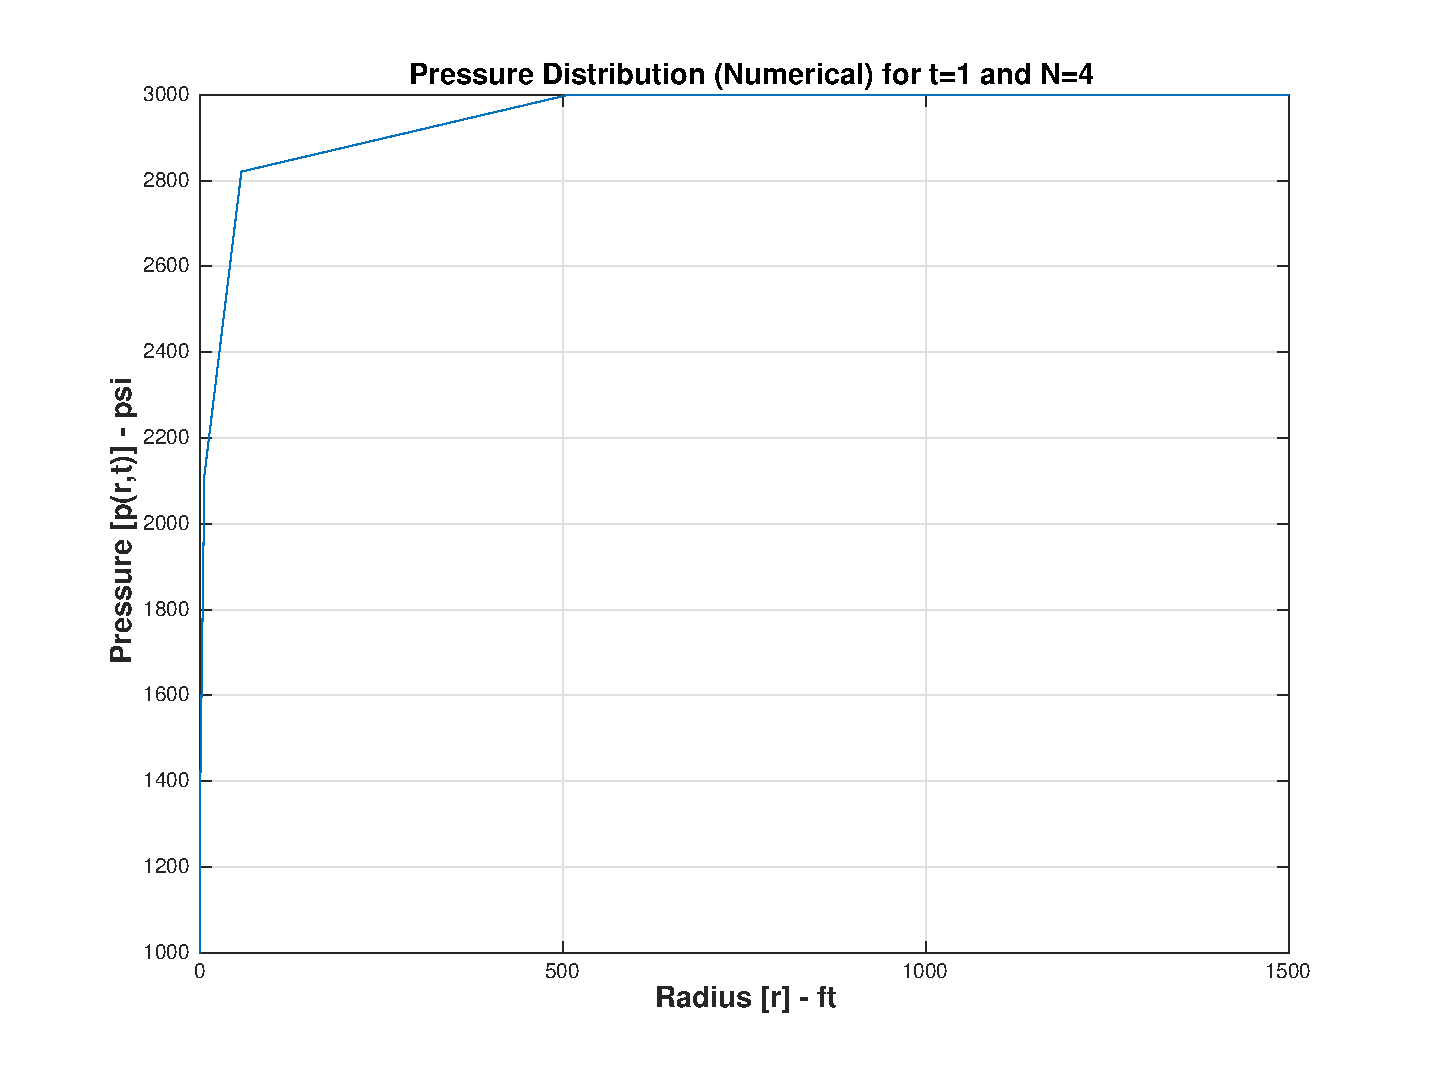
\includegraphics[width=1.5\textwidth]{P1_fig1.eps}}
\caption{\label{fig:3}Pressure Distribution for scenario 1}
\end{figure}
\begin{figure}[p]
\centering
\makebox[\textwidth][c]{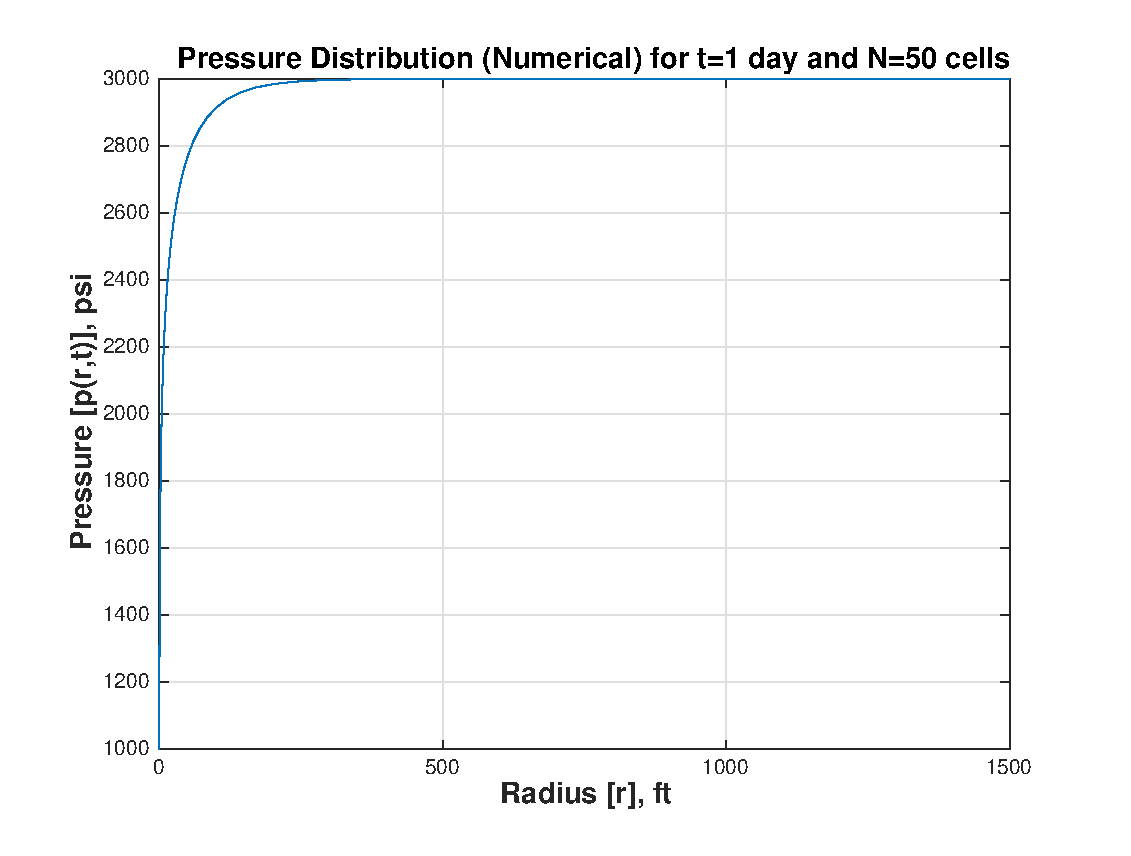
\includegraphics[width=1.5\textwidth]{n50t1.eps}}
\caption{\label{fig:50n}Pressure Distribution for 50 blocks after 1 day of production}
\end{figure}
\begin{figure}[p]
\centering
\makebox[\textwidth][c]{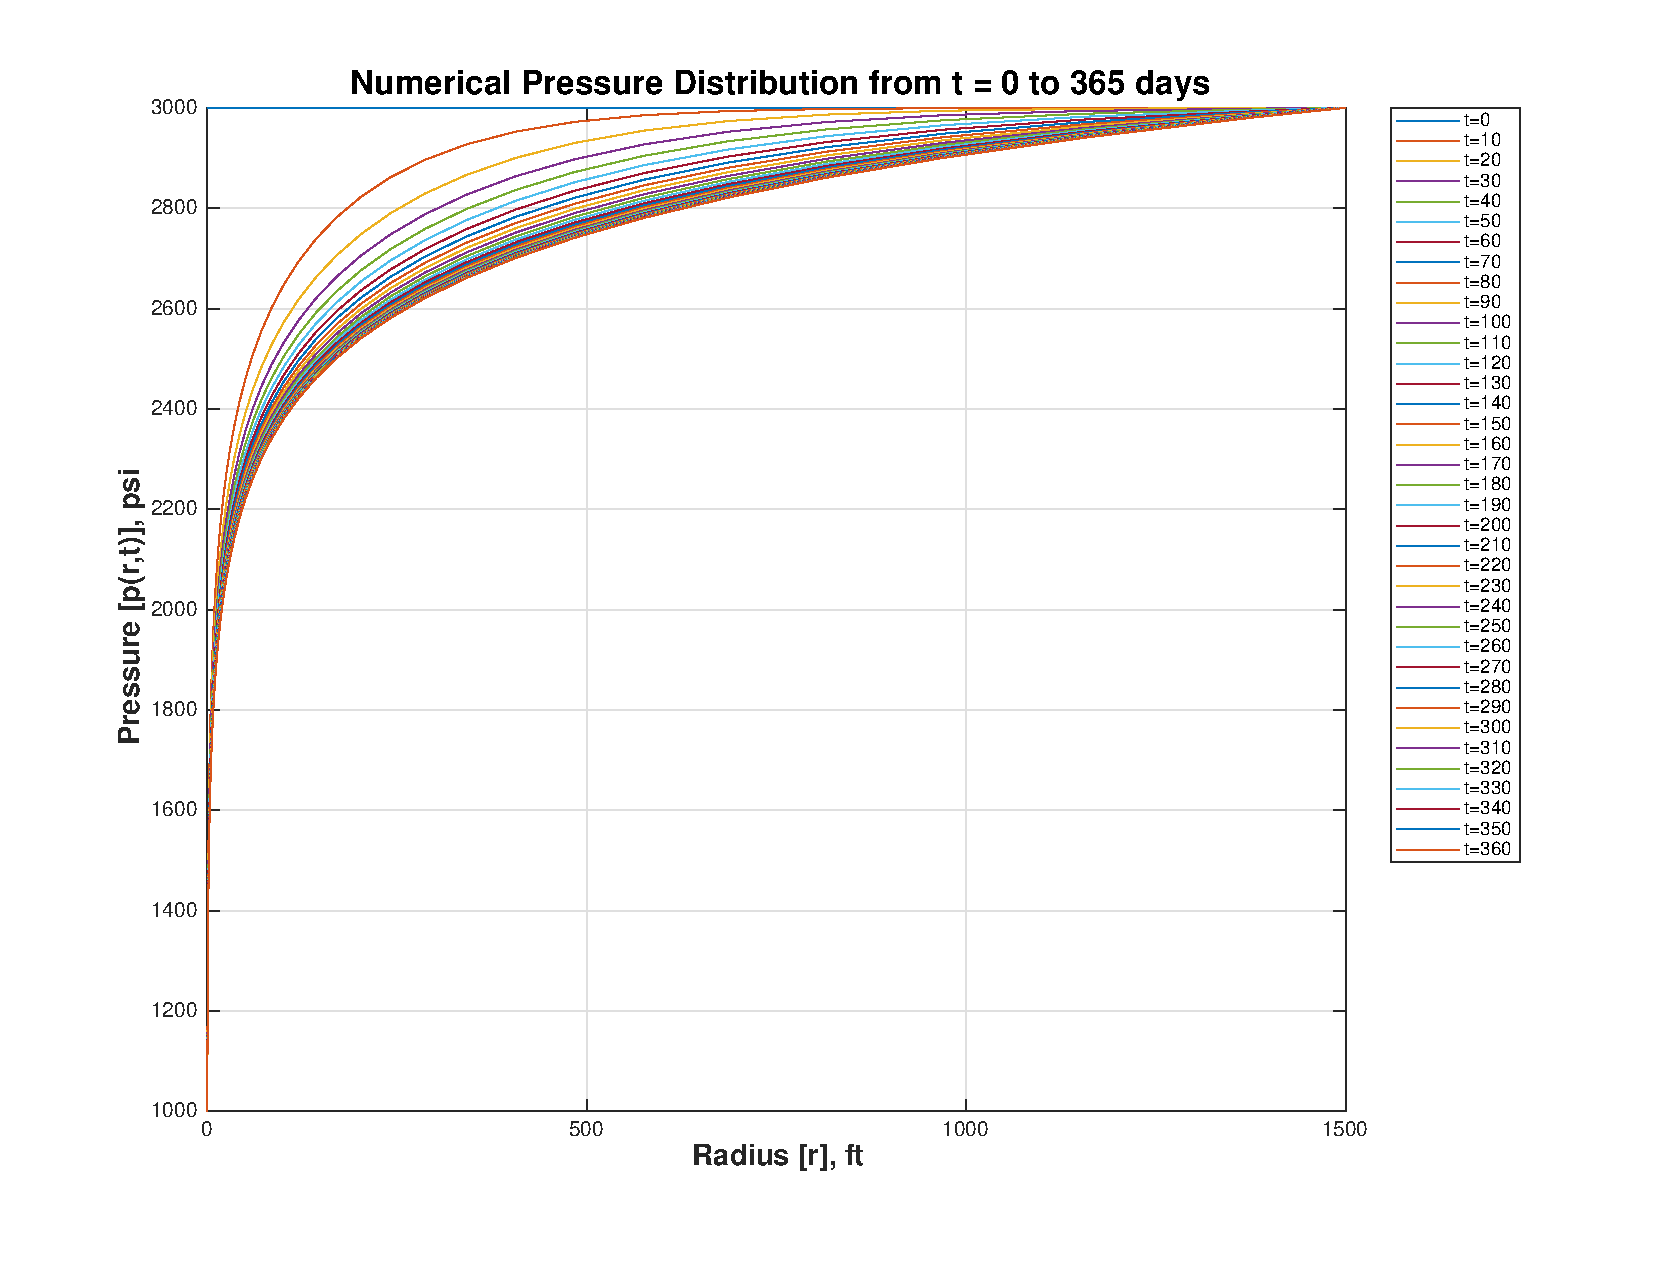
\includegraphics[width=1.5\textwidth]{Num__1_.eps}}
\caption{\label{fig:num}Pressure distribution for scenario 2}
\end{figure}
\begin{figure}[p]
\makebox[\textwidth][c]{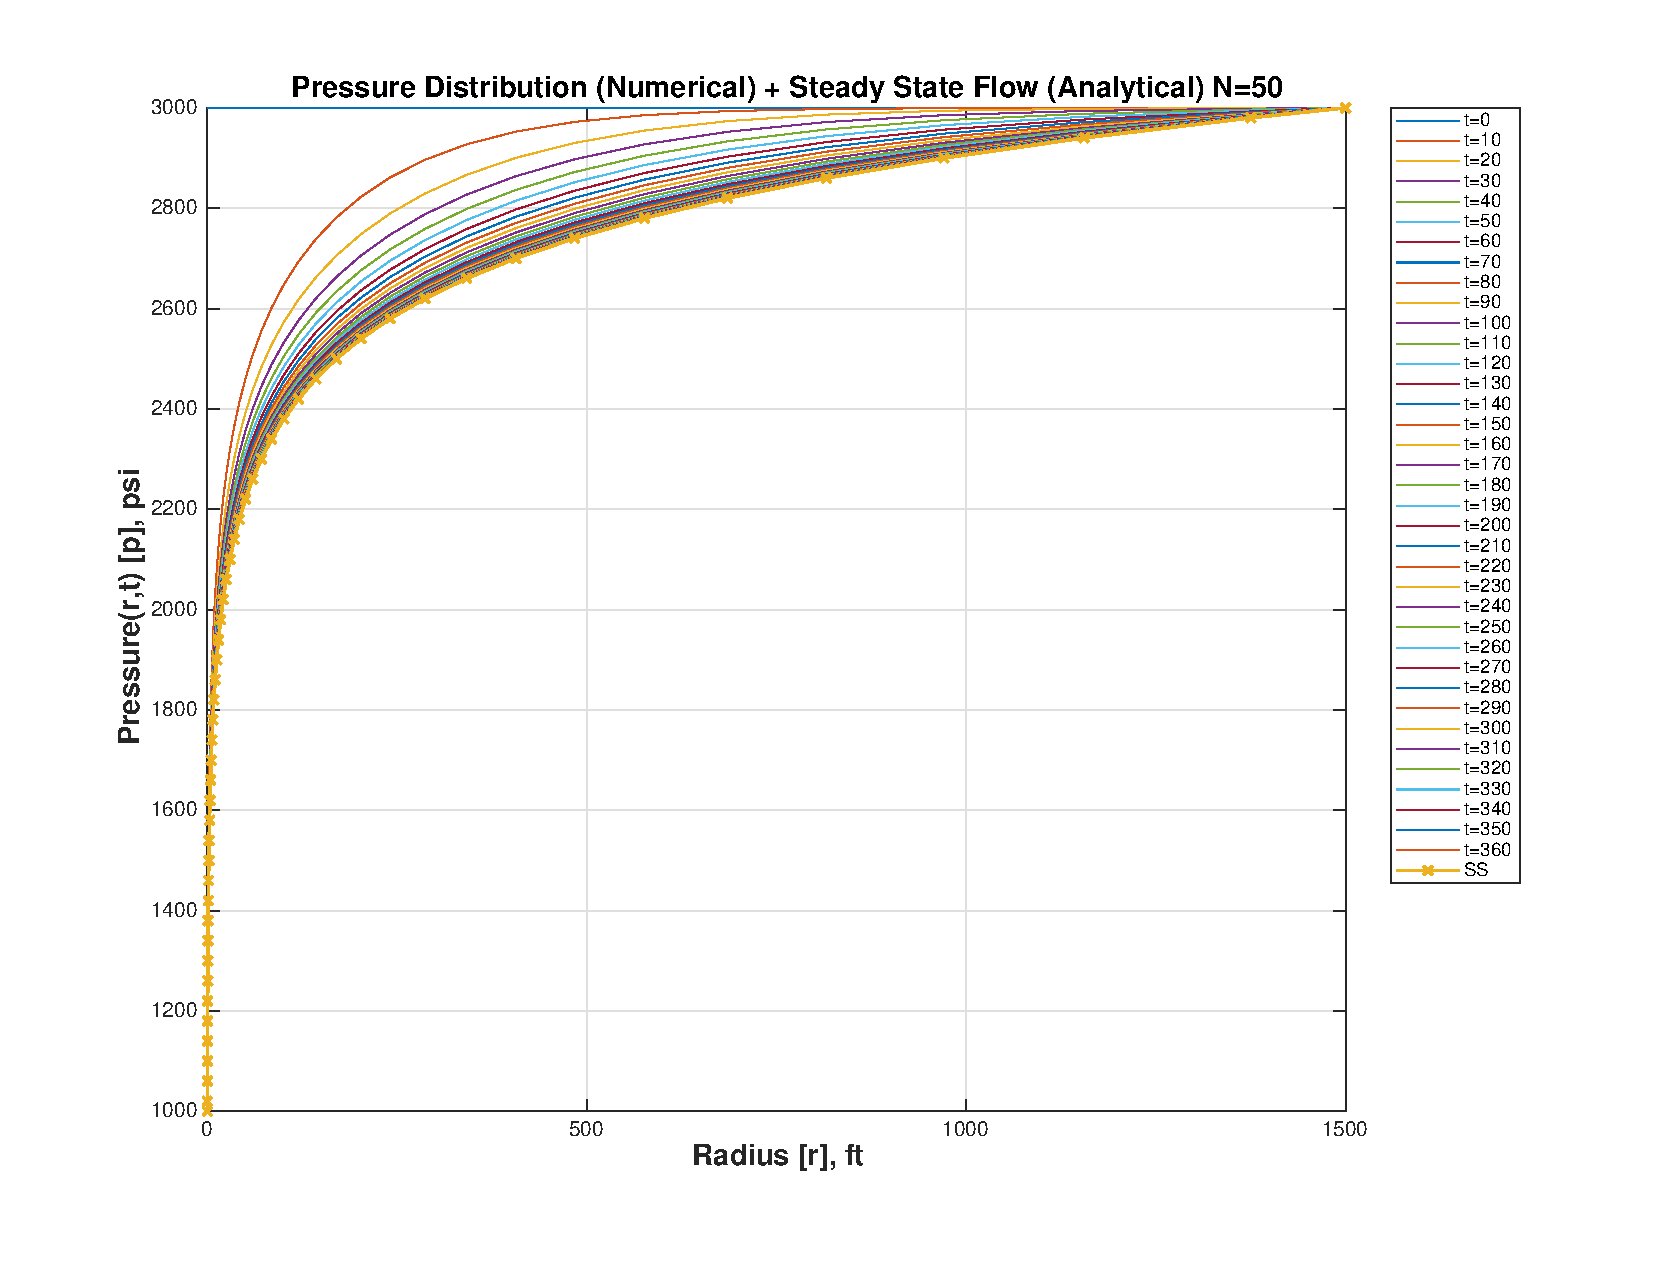
\includegraphics[width=1.5\textwidth]{Num+anal__1_.eps}}
\caption{\label{fig:numanal}Pressure Distribution for scenario 2 showing analytical steady state pressure}
\end{figure}

\begin{figure}[p]
\makebox[\textwidth][c]{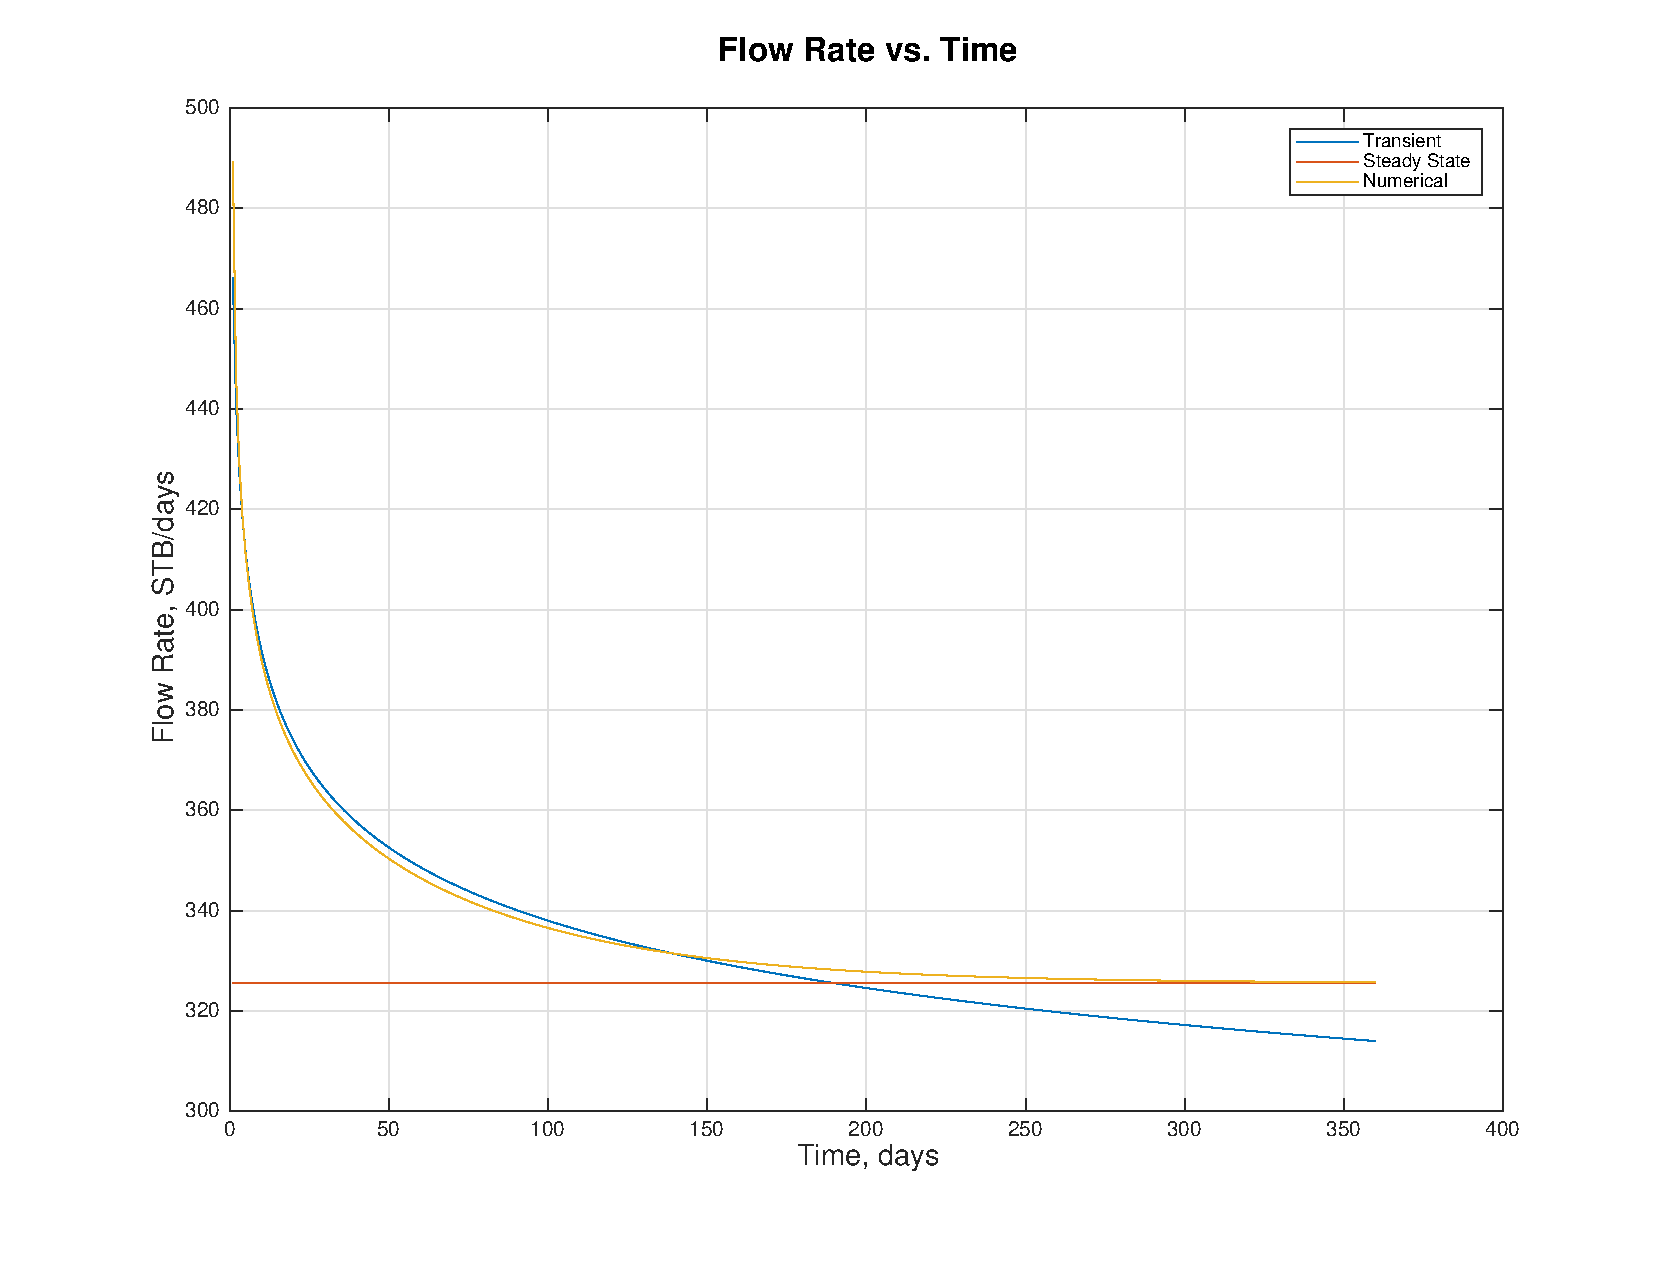
\includegraphics[width=1.5\textwidth]{SS__1_.eps}}
\caption{\label{fig:rate}Rate forecast using numerical method and analytical method for transit and steady state flows}
\end{figure}


\pagebreak
\appendix
Matlab R2017a code:
\begin{verbatim}
clc
clear all
%to solve for Part 1-5, make n=4 and t=1
t=360;
n=50;
%initial variables
re=1500;
rw=.25;
h=50;
pi=3000;
pwf=1000;
pe=3000;
k=10;
phi=.2;
vis=2;
B=1.25;
cf=1e-5;
co=2e-5;
dt=1;
S=0;
%assume variables for simplifying
ct=co+cf;
dx=(log(re)-log(rw))/n;
alpha= 158*phi*vis*ct/k;
ts=t/dt; %timestep
%create Pi array
for i=1:n
%    for j=1:ts
        pi(i) = 3000;
%    end
end
%create X & r arrays

% for m=1:ts
    for i=1:n
    x(i) = log(rw)+(2*i-1)/2*dx;
    end
% end
r=[rw,exp(x),re];
%defining discretized pressure coefficients (a,b,c,d)
% a Pi-1
for i=2:n-1
    a(i)=1;
end
a(n)=4;
%b Pi
b = -(2+alpha*dx^2/dt*exp(2*x));
b(1)= -(12+3*alpha*dx^2/dt*exp(2*x(1)));
b(n)= -(12+3*alpha*dx^2/dt*exp(2*x(n)));
%c Pi+1
for i=2:n-1
    c(i)=1;
end
c(1)=4;

d = ones(ts,n);
%time step
for m=1:ts
    d(m,1)= -3*alpha*exp(2*x(1,1))*dx^2/dt*pi(1,1)-8*pwf;
    d(m,n)= -3*alpha*exp(2*x(1,n))*dx^2/dt*pi(1,n)-8*pe;
    for i=2:n-1   
        %d RHS
        d(m,i) = -alpha*exp(2*x(1,i))*dx^2/dt*pi(1,i);
    end
    p_num=Thomas(a,b,c,d(m,:));
    press(m,:)=p_num;
    pi(1,:)=p_num;
end

p0=3000*ones(1,1*n+2);
p_pwf=pwf*ones(ts,1);
p_pe=pe*ones(ts,1);
press=[p_pwf,press,p_pe];
% P(r) calculations for steady state flow 
p_anal = pwf + ((pe-pwf)/(log(re/rw)))*log(r/rw);



%plotting
figure(1)
if (t==1)
    plot(r,press)
    title('Pressure Distribution (Numerical) for t=1 day and N=4 cells','fontsize',14,'fontweight','bold');
    xlabel('Radius [r], ft','fontsize',14,'fontweight','bold')
    ylabel('Pressure [p(r,t)], psi','fontsize',14,'fontweight','bold')
    grid on
else
    plot(r,p0,'DisplayName','t=0')
    hold on
    for i=1:t/10
        plot(r, press(i*10,:),'DisplayName',strcat('t=',num2str(i*10)))
        hold on 
    end
    hold off
    title('Numerical Pressure Distribution from t = 0 to 365 days','fontsize',16,'fontweight','bold')
    xlabel('Radius [r], ft','fontsize',14,'fontweight','bold')
    ylabel('Pressure [p(r,t)], psi','fontsize',14,'fontweight','bold')
    legend('show','location','northeastoutside')
    grid on

%plotting with SS
figure(2)

plot(r,p0,'DisplayName','t=0')
hold on
for i=1:t/10
    plot(r, press(i*10,:),'DisplayName',strcat('t=',num2str(i*10)))
    hold on 
end
plot(r,p_anal,'-x','linewidth',1.25,'DisplayName','SS')
hold off
title('Pressure Distribution (Numerical) + Steady State Flow (Analytical) N=50','fontsize',14,'fontweight','bold')
xlabel('Radius [r], ft','fontsize',14,'fontweight','bold')
ylabel('Pressure(r,t) [p], psi','fontsize',14,'fontweight','bold')
legend('show','location','northeastoutside')
grid on



%Step 9 - Rate Calculation using numerical simulation
for m=1:t
    q_num(m) = 7.08E-3*((k*h)/(vis*B))*((press(m,2)-pwf)/(0.5*dx));
end

%Flow Rate Calculation using Numerical Average Pressures (part 2 & 3)
for m=1:t
    tD(m) = (k*(m))/(158*phi*vis*(ct)*rw^2);
    y(m) = 1/(4*tD(m));
    pD(m) = -0.5*ei(-y(m));
    q_trans(m) = (7.08e-3*(k*h)/(vis*B))*((pe-pwf)/pD(m));
    
    q_ss(m) = 7.08E-3*((k*h)/(B*vis))*((pe-pwf)/(log(re/rw)+S));
end
t = [1:1:t];

% Flow Rate vs. Time plot
figure(3)
plot(t,q_trans,'DisplayName','Transient');
hold on
plot(t,q_ss,'DisplayName','Steady State');
hold on
plot(t,q_num,'DisplayName','Numerical');
legend('show')
hold off
xlabel('Time, days','FontSize', 14);
ylabel('Flow Rate, STB/days','FontSize', 14);
title({'Flow Rate vs. Time',' '},'FontSize', 16);
grid on
end
\end{verbatim}
\end{document}